% Tutorial @ https://www.overleaf.com/learn/latex/Learn_LaTeX_in_30_minutes

\documentclass[12pt, a4paper]{report}
\usepackage[utf8]{inputenc}
\usepackage{graphicx}
\usepackage{amsmath}
\usepackage[T1]{fontenc} % The T1 font encoding is an 8-bit encoding and uses fonts that have 256 glyphs. So an 'ö' is an actual single glyph in the font. The bigger problem is that without T1 you cannot copy/paste a name with a non-ascii glyph without getting them split up into their components.

\graphicspath{{images/}}
\title{Introduction to \LaTeX{}}
\author{Jovial Joe Jayarson \thanks{IES College of Engineering}}
\date{November 2020}

\begin{document}

\maketitle % This is needed for the title to be visible

\begin{abstract}
    This is a simple paragraph at the beginning of the document. A brief introduction about the main subject. The document contains the very basics of \LaTeX{} documentations. The tutorial is gratefully followed from Overleaf docs.
\end{abstract}

\tableofcontents

\chapter{\LaTeX{} 101} % \part and \chapter are only available in report and book document classes.

% To start a new line without actually starting a new paragraph insert a break line point, this can be done by \\ (a double backslash as in the example) or the \newline command.

% Care should be taken that multiple \\ or \newlines are not used to "simulate" paragraphs with larger spacing between them, as this can interfere with LaTeX's typesetting algorithms. The recommended method to do so is to keep using double blank lines to create new paragraphs without any \\, and then add \usepackage{parskip} to the preamble.

\section{Preamble, Paragraphs and Emphasis}

First document. This is a simple example, with no extra parameters or packages included. We have now added a title, author and date to our first \LaTeX{} document!

This line will start a second Paragraph.

% This line here is a comment, it will not be printed in the document.

Some of the \textbf{greatest} discoveries in \underline{science} were made by \textbf{\textit{accident}}. % What the \emph command actually does with its argument depends on the context - inside normal text the emphasized text is italicized, but this behavior is reversed if used inside an italicized text.

Some of the greatest \emph{discoveries} in science were made by accident.

\textit{Some of the greatest \emph{discoveries} in science were made by accident.}

\section{Images and Figures}

\subsection{Image}
The universe is immense and it seems to be homogeneous, in a large scale, everywhere we look at.

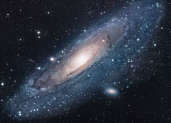
\includegraphics{universe} % no space between image names, good to omit extensions

There's a picture of a galaxy above.

\subsection{Figure}
\begin{figure}[h] % not sure of [h] exact meaning, but removing the same takes it beneath footer
    \centering
    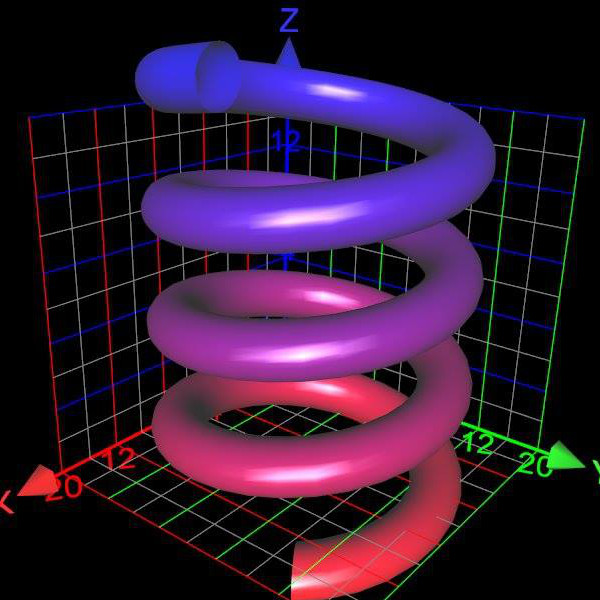
\includegraphics[width=0.25\textwidth]{graph}
    \caption{3D Circular Pipe}
    \label{fig:3D Torus}
\end{figure}

As you can see in the figure \ref{fig:3D Torus}, the function equivalent around 0. Also, in the page \pageref{fig:3D Torus}
is the same example.

\section{Lists}

Some unordered lists
\begin{itemize}
    \item The individual entries are indicated with a black dot, a so-called bullet.
    \item The text in the entires may be of any length.
\end{itemize}

Some ordered lists
\begin{enumerate}
    \item This is the first entry of the list
    \item The list number increases
    \item As each entry is added
\end{enumerate}

\section{Math in \LaTeX{}}

% Adding Math to LaTeX
In physics, the mass-energy equivalence is stated by the equation $E = mc^2$ discovered in 1905 by Albert Einstein. % same as \begin{math} ... \end{math}
In natural units ($c = 1$) the formula expresses the identity
\[ E = m \] % same as \begin{displaymath} ... \end{displaymath}
In mathematics the most beautiful equation is stated as
\begin{equation}
    e^{i\pi} + 1 = 0
\end{equation}

% $$ ... $$ is discouraged as it can give inconsistent spacing, and may not work well with some math packages.

% equation* environment is provided by an external package, [amsmath](https://www.overleaf.com/learn/Aligning_equations).

Subscripts in mathematics are written as $a_b$ and superscripts are written as $a^b$. These can be combined and nested to write equations such as:

\[ T^{i_1 i_2 \dots i_p}_{j_1 j_2 \dots j_q} = T(x^{i_1},\dots,x^{i_p},e_{j_1},\dots,e_{j_q}) \]

We write integral using using $\int$ and fractions using $\frac{a}{b}$. Limits are placed on integral using subscripts and superscripts.

\[ \int_0^1 \frac{dx}{e^x} =  \frac{e-1}{e} \]

Lower case Greek letters are written as $\omega$ $\delta$ etc. while upper case Greek letters are written as $\Omega$ $\Delta$.

Mathematical operators are prefixed with a backslash as $\sin(\beta)$, $\cos(\alpha)$, $\log(x)$ etc.

\section*{Unnumbered Section}
Lorem ipsum dolor sit amet, consectetuer adipiscing elit. Etiam lobortis facilisissem

\section{Creating Tables}

\subsection{Basic Tables}
\begin{center}
    \begin{tabular}{ c c c }
        cell1 & cell2 & cell3 \\
        cell4 & cell5 & cell6 \\
        cell7 & cell8 & cell9
    \end{tabular}
\end{center}

\subsection{Adding borders}
\begin{center}
    \begin{tabular}{ |c|c|c| }
        \hline
        cell1 & cell2 & cell3 \\
        cell4 & cell5 & cell6 \\
        cell7 & cell8 & cell9 \\
        \hline
    \end{tabular}
\end{center}

\begin{itemize}
    \item { | c | c | c | }: This declares that three columns, separated by a vertical line, are going to be used in the table. The | symbol specifies that these columns should be separated by a vertical line.
    \item \verb|\hline|: This will insert a horizontal line. We have included horizontal lines at the top and bottom of the table here. There is no restriction on the number of times you can use \verb|\hline|.
\end{itemize}

Creating tables in LaTeX can be a bit tricky sometimes, so you may want to use the TablesGenerator.com online tool to export LaTeX code for tables. The File > Paste table data option lets you copy and paste data from spreadsheet applications.

\begin{center}
    \begin{tabular}{||c c c c||}
        \hline
        Col1 & Col2 & Col2  & Col3 \\ [0.5ex]
        \hline\hline
        1    & 6    & 87837 & 787  \\
        \hline
        2    & 7    & 78    & 5415 \\
        \hline
        3    & 545  & 778   & 7507 \\
        \hline
        4    & 545  & 18744 & 7560 \\
        \hline
        5    & 88   & 788   & 6344 \\ [1ex]
        \hline
    \end{tabular}
\end{center}

\section{Captions, labels and references}

You can caption and reference tables in much the same way as images. The only difference is that instead of the figure environment, you use the table environment.

able \ref{table:data} is an example of referenced \LaTeX{} elements.

\begin{table}[h!]
    \centering
    \begin{tabular}{||c c c c||}
        \hline
        Col1 & Col2 & Col2  & Col3 \\ [0.5ex]
        \hline\hline
        1    & 6    & 87837 & 787  \\
        2    & 7    & 78    & 5415 \\
        3    & 545  & 778   & 7507 \\
        4    & 545  & 18744 & 7560 \\
        5    & 88   & 788   & 6344 \\ [1ex]
        \hline
    \end{tabular}
    \caption{Table to test captions and labels}
    \label{table:data}
\end{table}

\end{document}
